We begin our study by discussing the large time dependence observed in data and associated to the actual interval of time over which the LHC delivered luminosity to the ATLAS detector. 

Data is taken in small chunks, called LumiBlocks (LBs), with an average duration of about 60 sec. The distribution of LB durations across the entire Run~II data taking period (2015-2018) is shown in the left panel of figure~\ref{fig:LBs}. The total number of LBs during Run-II is summarized in Table~\ref{tab:LBs}.

\begin{figure}[H]
\centering
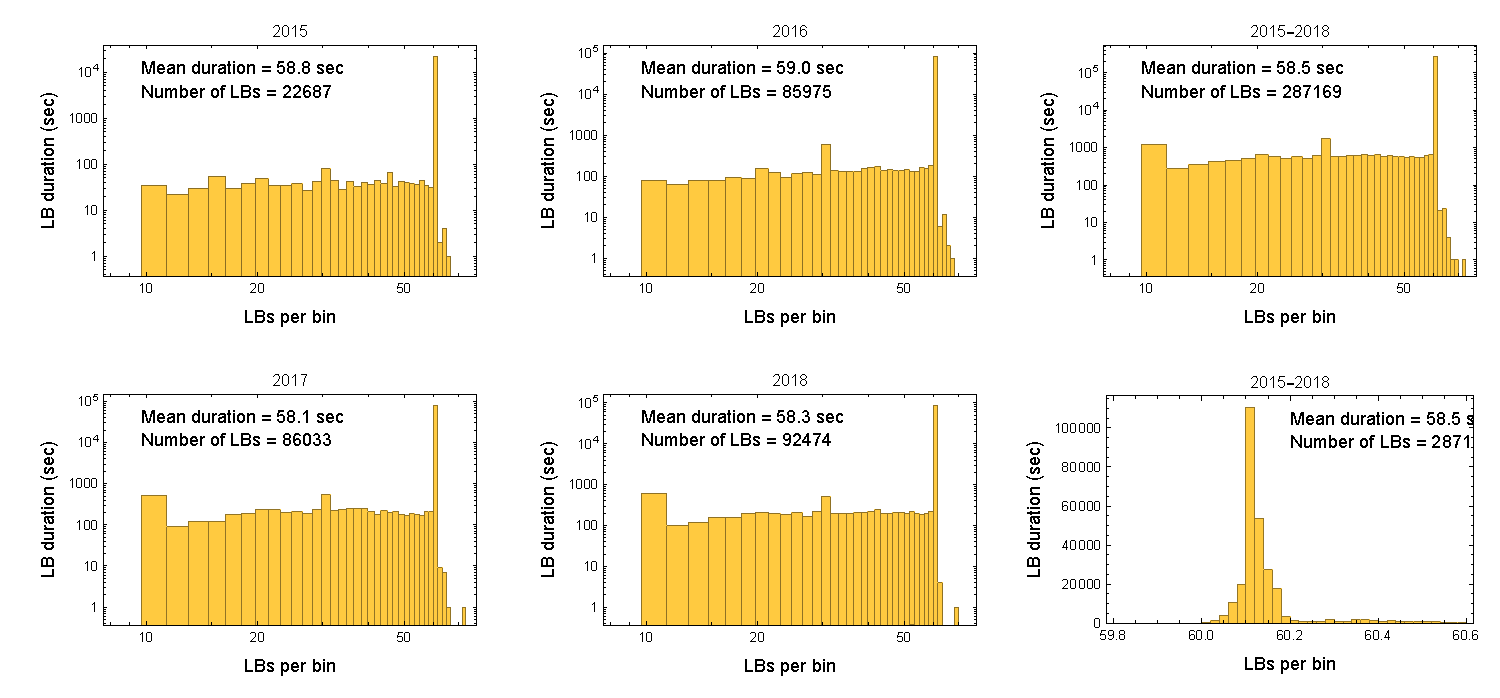
\includegraphics[width=\textwidth]{figs/Mathematica-oldchi2/LB_duration_log_allyears}
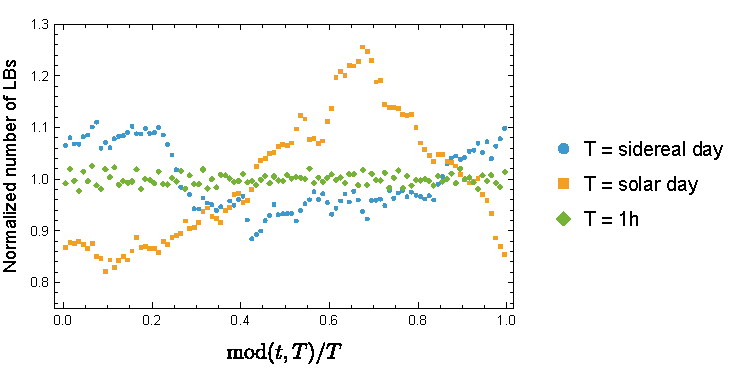
\includegraphics[width=0.7 \textwidth]{figs/Mathematica-oldchi2/LB_phase}
\caption{Distribution of the LumiBlocks durations (top panel) and phases (bottom panel) across the entire data taking period.}
\label{fig:LBs}
\end{figure}

\begin{table}[H]
    \centering
    \begin{tabular}{|c|c|} \hline
         Year & Number of LBs \\ \hline 
         2015 & 22687 \\
         2016 & 85975 \\
         2017 & 86033 \\
         2018 & 92474 \\ \hline
         total & 287169 \\ \hline
        \end{tabular}
    \caption{Yearly and total number of LBs in Run-II.}
    \label{tab:LBs}
\end{table}

Each LB has a unique time stamp which is taken to be the average of its initial and final time stamps. From this time stamp, the time in the Sun-Centered-Frame is constructed as discussed in Sec.~\ref{sec:timeshift}. Finally, for a giving testing period (e.g. solar day ($T = 24\text{hr}$), sidereal day ($T = 23.93\text{hr}$), \ldots), each time stamp, $t$, is converted to a phase in the interval $[0,1]$:
%
\begin{align}
t \rightarrow \phi (T) = \text{mod}[ t , T ]/T  \; .  
\end{align}
%
In the right panel of figure~\ref{fig:LBs} we show the normalized distribution of the LBs phases calculated using three testing periods: $T_\text{solar}$, $T_\text{sidereal}$ and $T = 1 \text{hr}$. As can be seen there is a very large solar day dependence, with much more data taken near $\phi (T_\text{solar}) \sim 0.7$ which corresponds to the middle of the night in Geneva (about $4\text{am}$).  

In figure~\ref{fig:Lumi_phase} we show the normalized distribution of the integrated Luminosity across the four data taking years. The pattern of peak luminosity recorded in the middle of the night is consistent across the four years. The 2015-2018 cumulative distribution is essentially identical to the LB distribution presented in figure~\ref{fig:LBs}.

\begin{figure}[H]
\centering
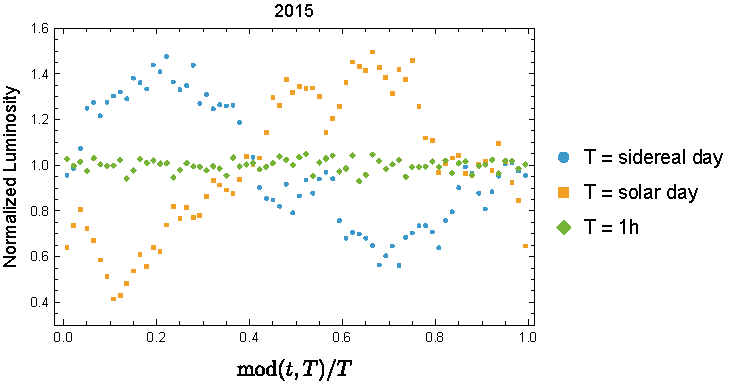
\includegraphics[width=0.49\textwidth]{figs/Mathematica-oldchi2/Lumi_phase_2015}
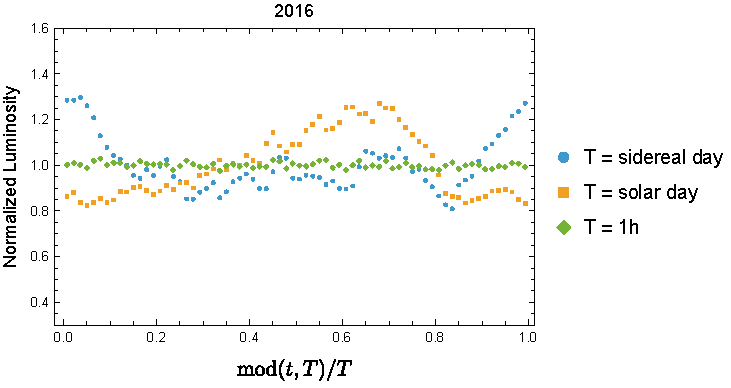
\includegraphics[width=0.49\textwidth]{figs/Mathematica-oldchi2/Lumi_phase_2016}
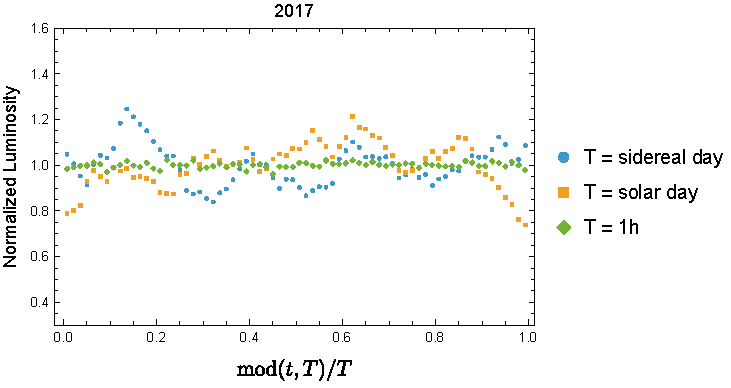
\includegraphics[width=0.49\textwidth]{figs/Mathematica-oldchi2/Lumi_phase_2017}
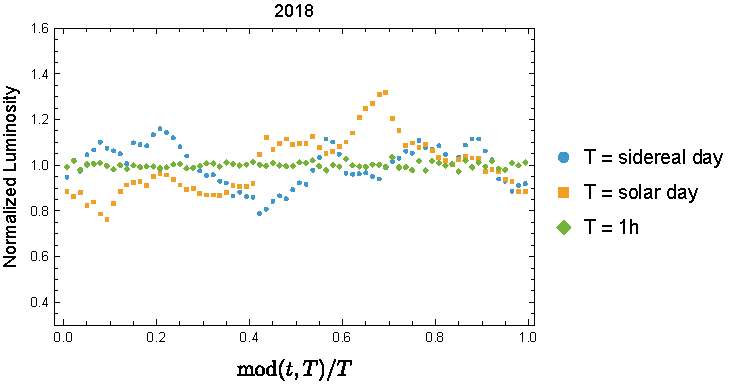
\includegraphics[width=0.49\textwidth]{figs/Mathematica-oldchi2/Lumi_phase_2018}
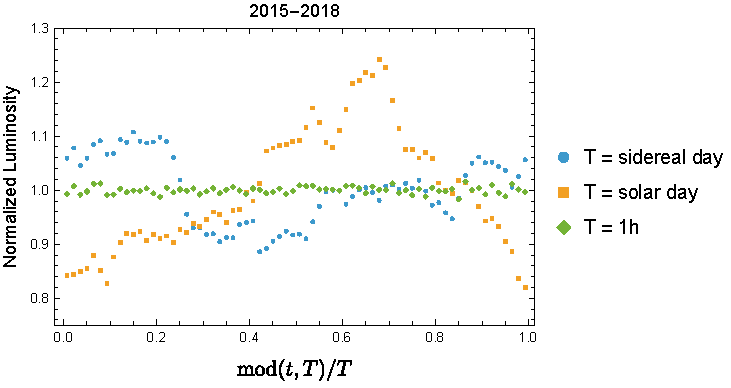
\includegraphics[width=0.49\textwidth]{figs/Mathematica-oldchi2/Lumi_phase_allyears}
\caption{Normalized distribution of the integrated Luminosity as a function of the phase for the four data taking years.}
\label{fig:Lumi_phase}
\end{figure}

In the next step, we construct time distributions of simulated $Z$ counts. For each LB, we combine time stamp, efficiency ($\varepsilon$), Monte Carlo correction factor ($F_\text{MC}(\mu)$ with $\mu$ taken from data) and luminosity with the fiducial NNLO SM cross section:
%
\begin{align}
N_\text{fid}^\text{SM} (t) = \sigma_\text{SM}\cdot  A_\text{SM}\cdot \varepsilon(t) \cdot  F_\text{MC} (\mu(t)) \cdot {\cal L}_\text{inst}(t) \cdot \Delta t
\label{eq:NZsim}
\end{align}
%
where all time dependent quantities are taken from data. The resulting normalized distribution as a function of phase is shown in the left panel of figure~\ref{fig:NZsimulated}. We also Poisson sampled each $N_\text{fid}^\text{SM} (t)$ and constructed the corresponding normalized distribution, which is presented in the right panel of figure~\ref{fig:NZsimulated}.

\begin{figure}[H]
\centering
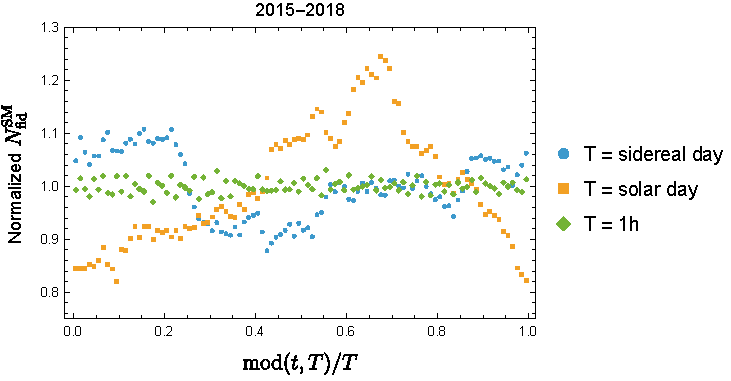
\includegraphics[width=0.49\textwidth]{figs/Mathematica-oldchi2/Nfiducial_theory_phase}
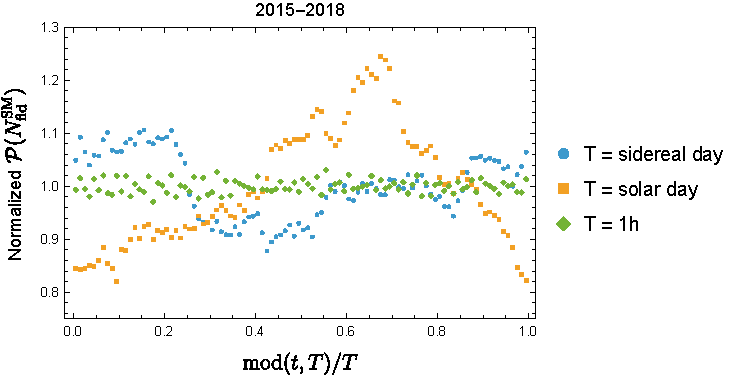
\includegraphics[width=0.49\textwidth]{figs/Mathematica-oldchi2/Nfiducial_theory(Poisson)_phase}
\caption{Normalized distribution of simulated $Z$ counts. Time stamps, Luminosity and efficiencies are taken from data. The left panel is obtained from the central values of the simulated Z counts in each LB ($N_\text{fid}^\text{SM}$). The right panel is obtained by Poisson sampling Z counts in each LB (${\cal P} (N_\text{fid}^\text{SM})$).}
\label{fig:NZsimulated}
\end{figure}

From this preliminary distributions it is clear that the data has a strong time dependence which is completely dominated by the actual data taking pattern. In the next section we begin exploring the time distribution of the cross section measured in each LB which is expected to be free from these effect. 